\begin{ujnbody}
    \section{基础功能测试(节标题section)}
    \subsection{文字(子节标题subsection)}
    这是文字。
    \subsubsection{段落(子小节标题subsubsection)}
    这是段落。这是段落。这是段落。这是段落。这是段落。这是段落。这是段落。这是段落。这是段落。这是段落。这是段落。这是段落。这是段落。这是段落。这是段落。这是段落。这是段落。这是段落。这是段落。这是段落。

    这是另一个段落。这是另一个段落。这是另一个段落。这是另一个段落。这是另一个段落。这是另一个段落。这是另一个段落。这是另一个段落。这是另一个段落。这是另一个段落。这是另一个段落。这是另一个段落。这是另一个段落。
    \subsection{图表与代码块}
    \subsubsection{图片}
    \begin{figure}[htbp]
        \centering
        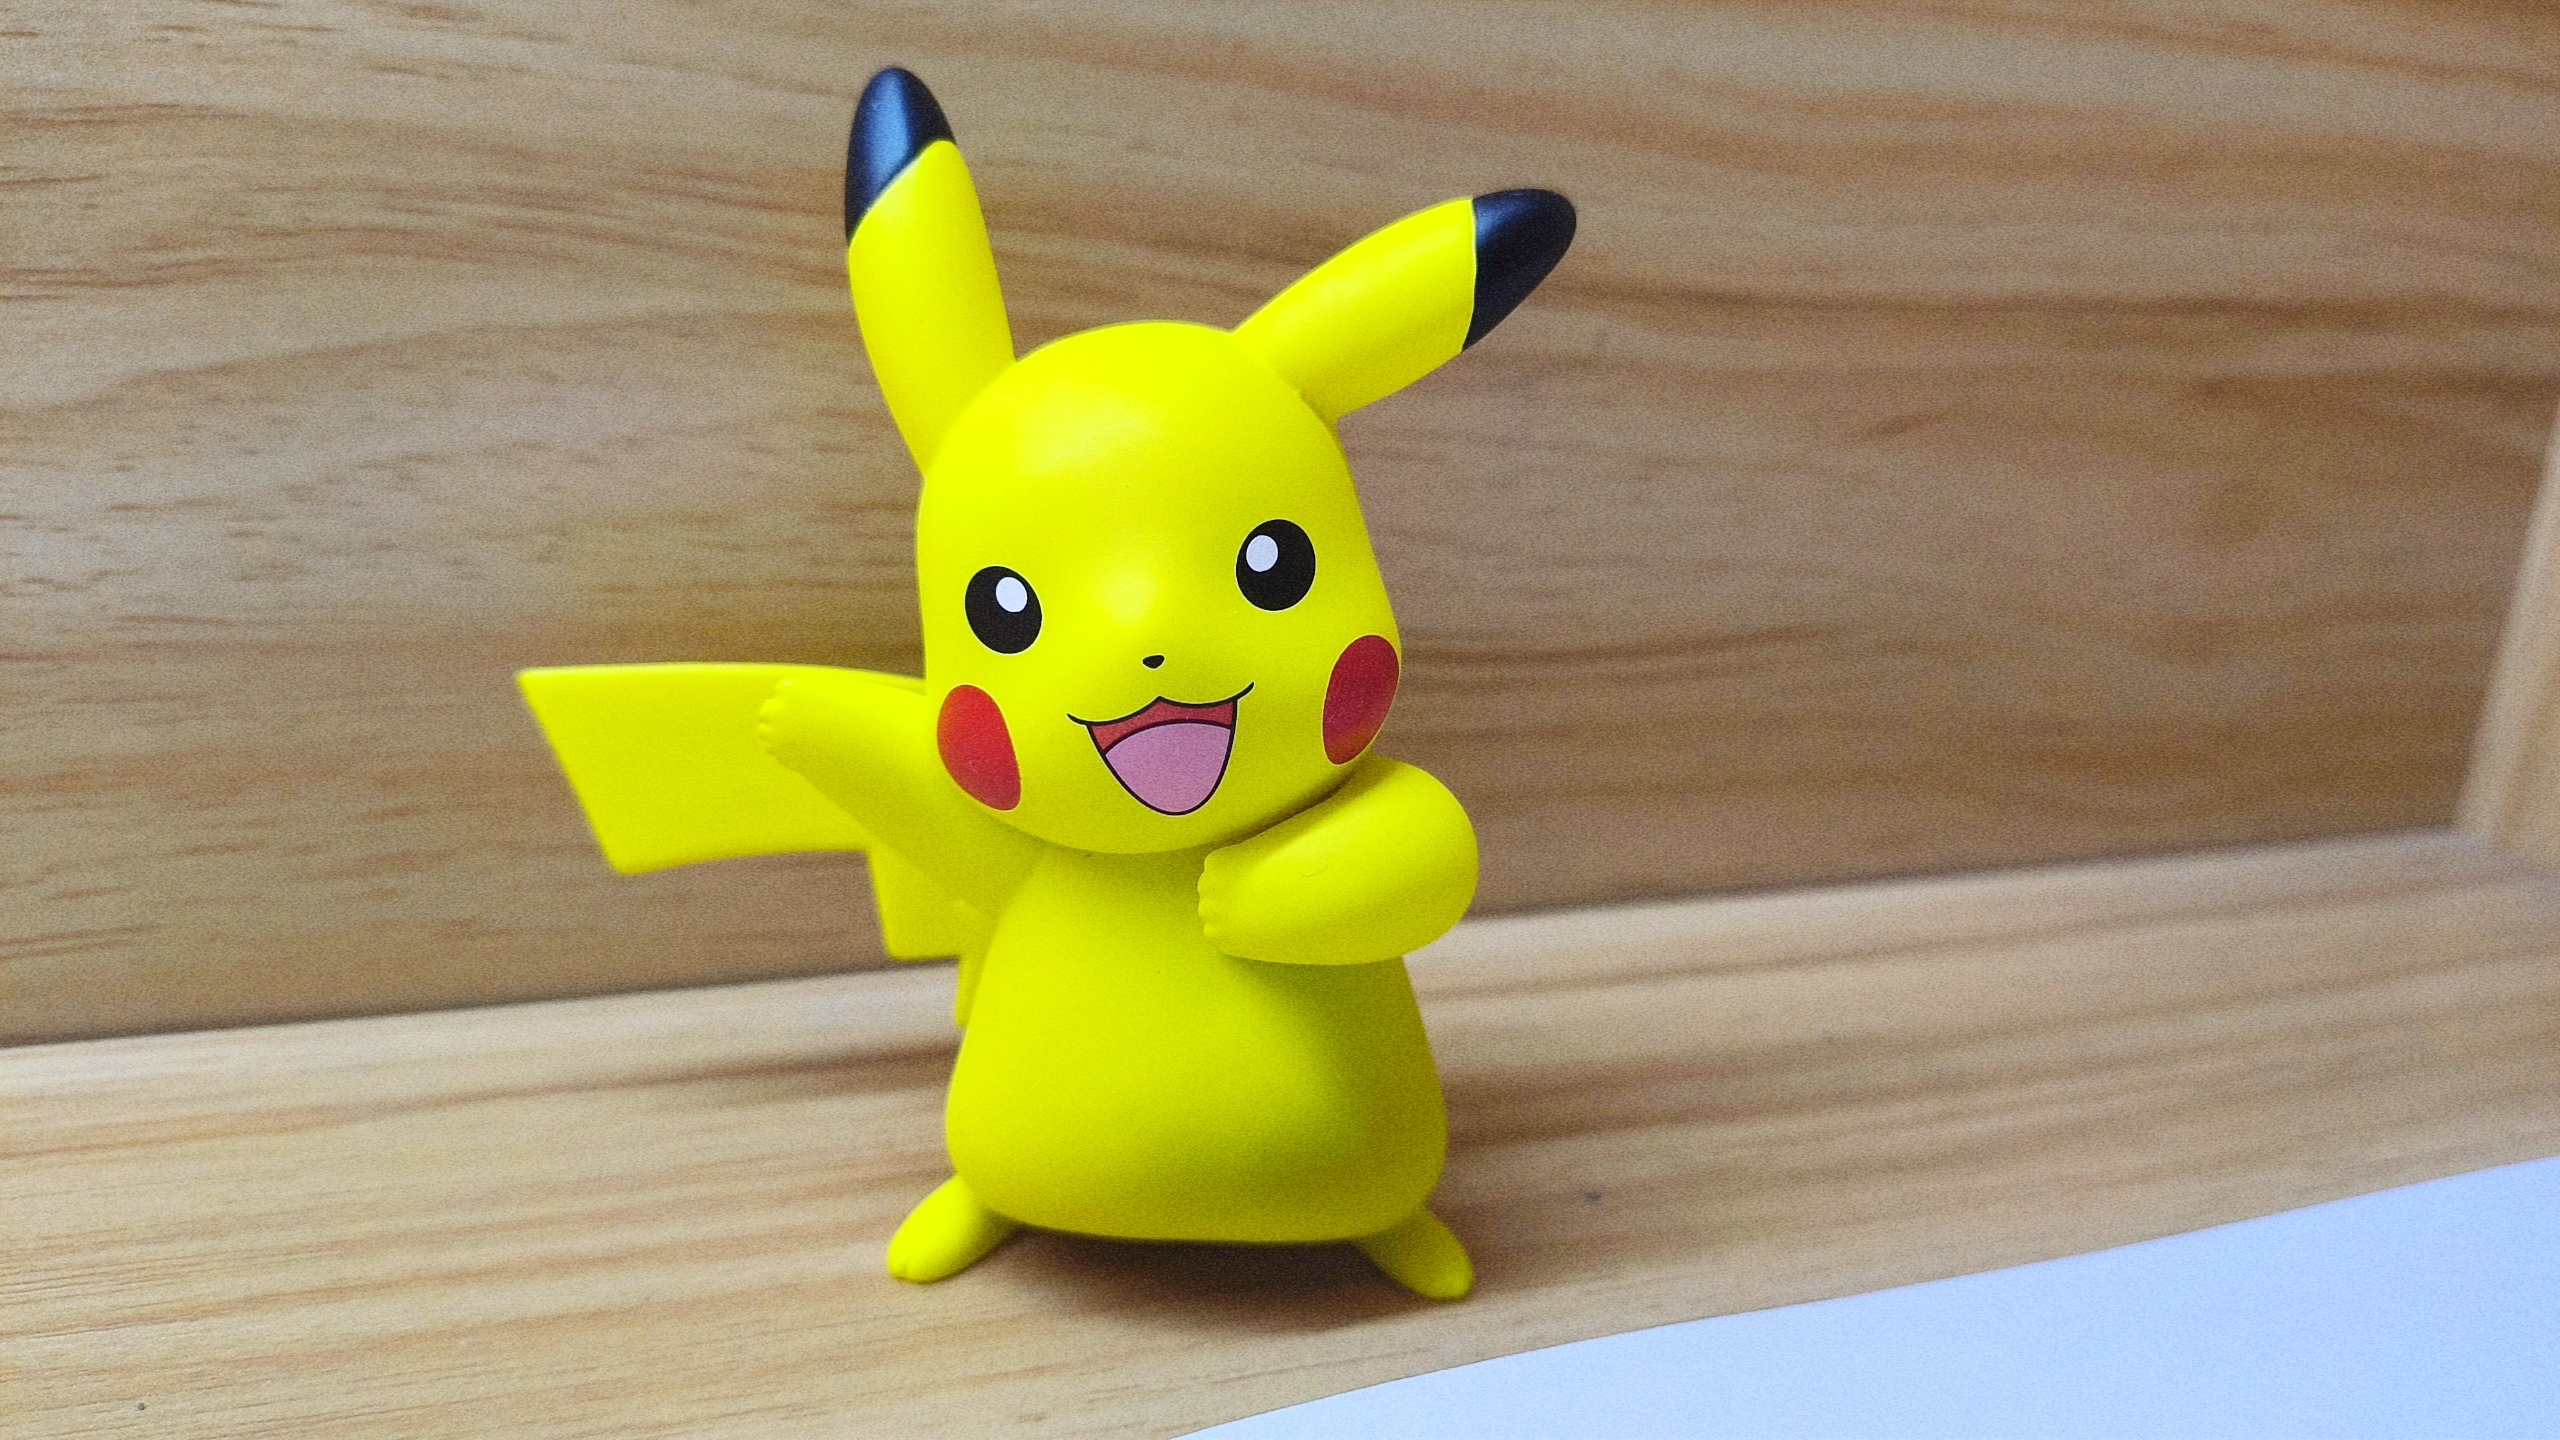
\includegraphics[scale=0.1]{figures/pikachu.jpg}
        \caption{这是图片}
        \label{fig:1}
    \end{figure}
    \subsubsection{表格}
    \begin{table}[!htbp]
        \centering
        \caption{这是表格}
        \begin{tabular}{cccccc}
            \toprule
            序号 & 姓名 & 性别 & 年龄 & 身高/cm & 体重/kg \\
            \midrule
            1 & 张三 & M & 16 & 163 & 50 \\
            2 & 王红 & F & 15 & 159 & 47 \\
            3 & 李二 & M & 17 & 165 & 52 \\
            \bottomrule
        \end{tabular}
        \label{tab:1}
    \end{table}
    \subsubsection{代码块}
    \begin{lstlisting}
        #include <stdio.h>
        /* hello,world */
        int main(){
            printf("Hello, World! \n"); 
            return 0;
        }
    \end{lstlisting}
    \subsection{数学公式}
    \subsubsection{行内公式}
    这是简单的行内公式:$x^2+y^2=z^2$,这是复杂的行内公式:$\sum_{i=1}^n a_i=0$。
    \subsubsection{行间公式}
    (1)线性代数部分:
    \begin{equation}
        \begin{split}
            \mathbf{A}\mathbf{x} &= \mathbf{b} \\
            \mathbf{A}^{-1}\mathbf{A}\mathbf{x} &= \mathbf{A}^{-1}\mathbf{b} \\
            \mathbf{I}\mathbf{x} &= \mathbf{A}^{-1}\mathbf{b} \\
            \mathbf{x} &= \mathbf{A}^{-1}\mathbf{b}
        \end{split}
    \end{equation}

    (2)微积分部分:
    \begin{equation}
        \begin{split}
            \frac{d}{dx} \int_a^x f(t)\,dt &= f(x) \label{eq:1} \\
            \int_a^b f(x)\,dx &= F(b)-F(a)
        \end{split}
    \end{equation}

    (3)概率论部分:
    \begin{equation}
        \begin{split}
            P(A \mid B) &= \frac{P(A \cap B)}{P(B)} \\
            &= \frac{P(B \cap A)}{P(B)} \\
            &= \frac{P(B \mid A)P(A)}{P(B)}
        \end{split}
    \end{equation}

    (4)统计部分:
    \begin{equation}
        \begin{split}
            \bar{x} &= \frac{1}{n}\sum_{i=1}^n x_i \\
            s^2 &= \frac{1}{n-1}\sum_{i=1}^n (x_i-\bar{x})^2 \\
            s &= \sqrt{s^2}
        \end{split}
    \end{equation}

    (5)离散数学部分:
    \begin{equation}
        \begin{split}
            \binom{n}{k} &= \frac{n!}{k!(n-k)!} \\
            \binom{n}{0} &= \binom{n}{n} = 1 \\
            \binom{n}{1} &= \binom{n}{n-1} = n \\
            \binom{n}{2} &= \binom{n}{n-2} = \frac{n(n-1)}{2} \\
            \binom{n}{k} &= \binom{n}{n-k}
        \end{split}
    \end{equation}

    (6)其他部分:
    \begin{equation}
        \begin{split}
            \log_a x &= \frac{\log_b x}{\log_b a} \\
            \log_a x &= \frac{\log_c x}{\log_c a} \\
            \log_a x &= \frac{\log_a b}{\log_a c} \\
            \log_a x &= \frac{\log_b x}{\log_b c}
        \end{split}
    \end{equation}
    \section{交叉引用}\label{sec:1}
    \subsection{参考文献引用}\label{sec:2}
    这是第一个参考文献的交叉引用\cite{shannon1948mathematical}。

    这是第二个参考文献的交叉引用\cite{nash1996non}。

    这是第三个参考文献的交叉引用\cite{turing2009computing}。
    \subsection{图表引用}
    这是图片\ref{fig:1}的交叉引用。

    这是表格\ref{tab:1}的交叉引用。
    \subsection{章节引用}
    这是章节\ref{sec:1}的交叉引用。

    这是章节\ref{sec:2}的交叉引用。
    \subsection{公式引用}
    这是公式\ref{eq:1}的交叉引用。
    \section{基础功能测试(节标题section)}
    \subsection{文字(子节标题subsection)}
    这是文字。
    \subsubsection{段落(子小节标题subsubsection)}
    这是段落。这是段落。这是段落。这是段落。这是段落。这是段落。这是段落。这是段落。这是段落。这是段落。这是段落。这是段落。这是段落。这是段落。这是段落。这是段落。这是段落。这是段落。这是段落。这是段落。

    这是另一个段落。这是另一个段落。这是另一个段落。这是另一个段落。这是另一个段落。这是另一个段落。这是另一个段落。这是另一个段落。这是另一个段落。这是另一个段落。这是另一个段落。这是另一个段落。这是另一个段落。
    \subsection{图表与代码块}
    \subsubsection{图片}
    \begin{figure}[htbp]
        \centering
        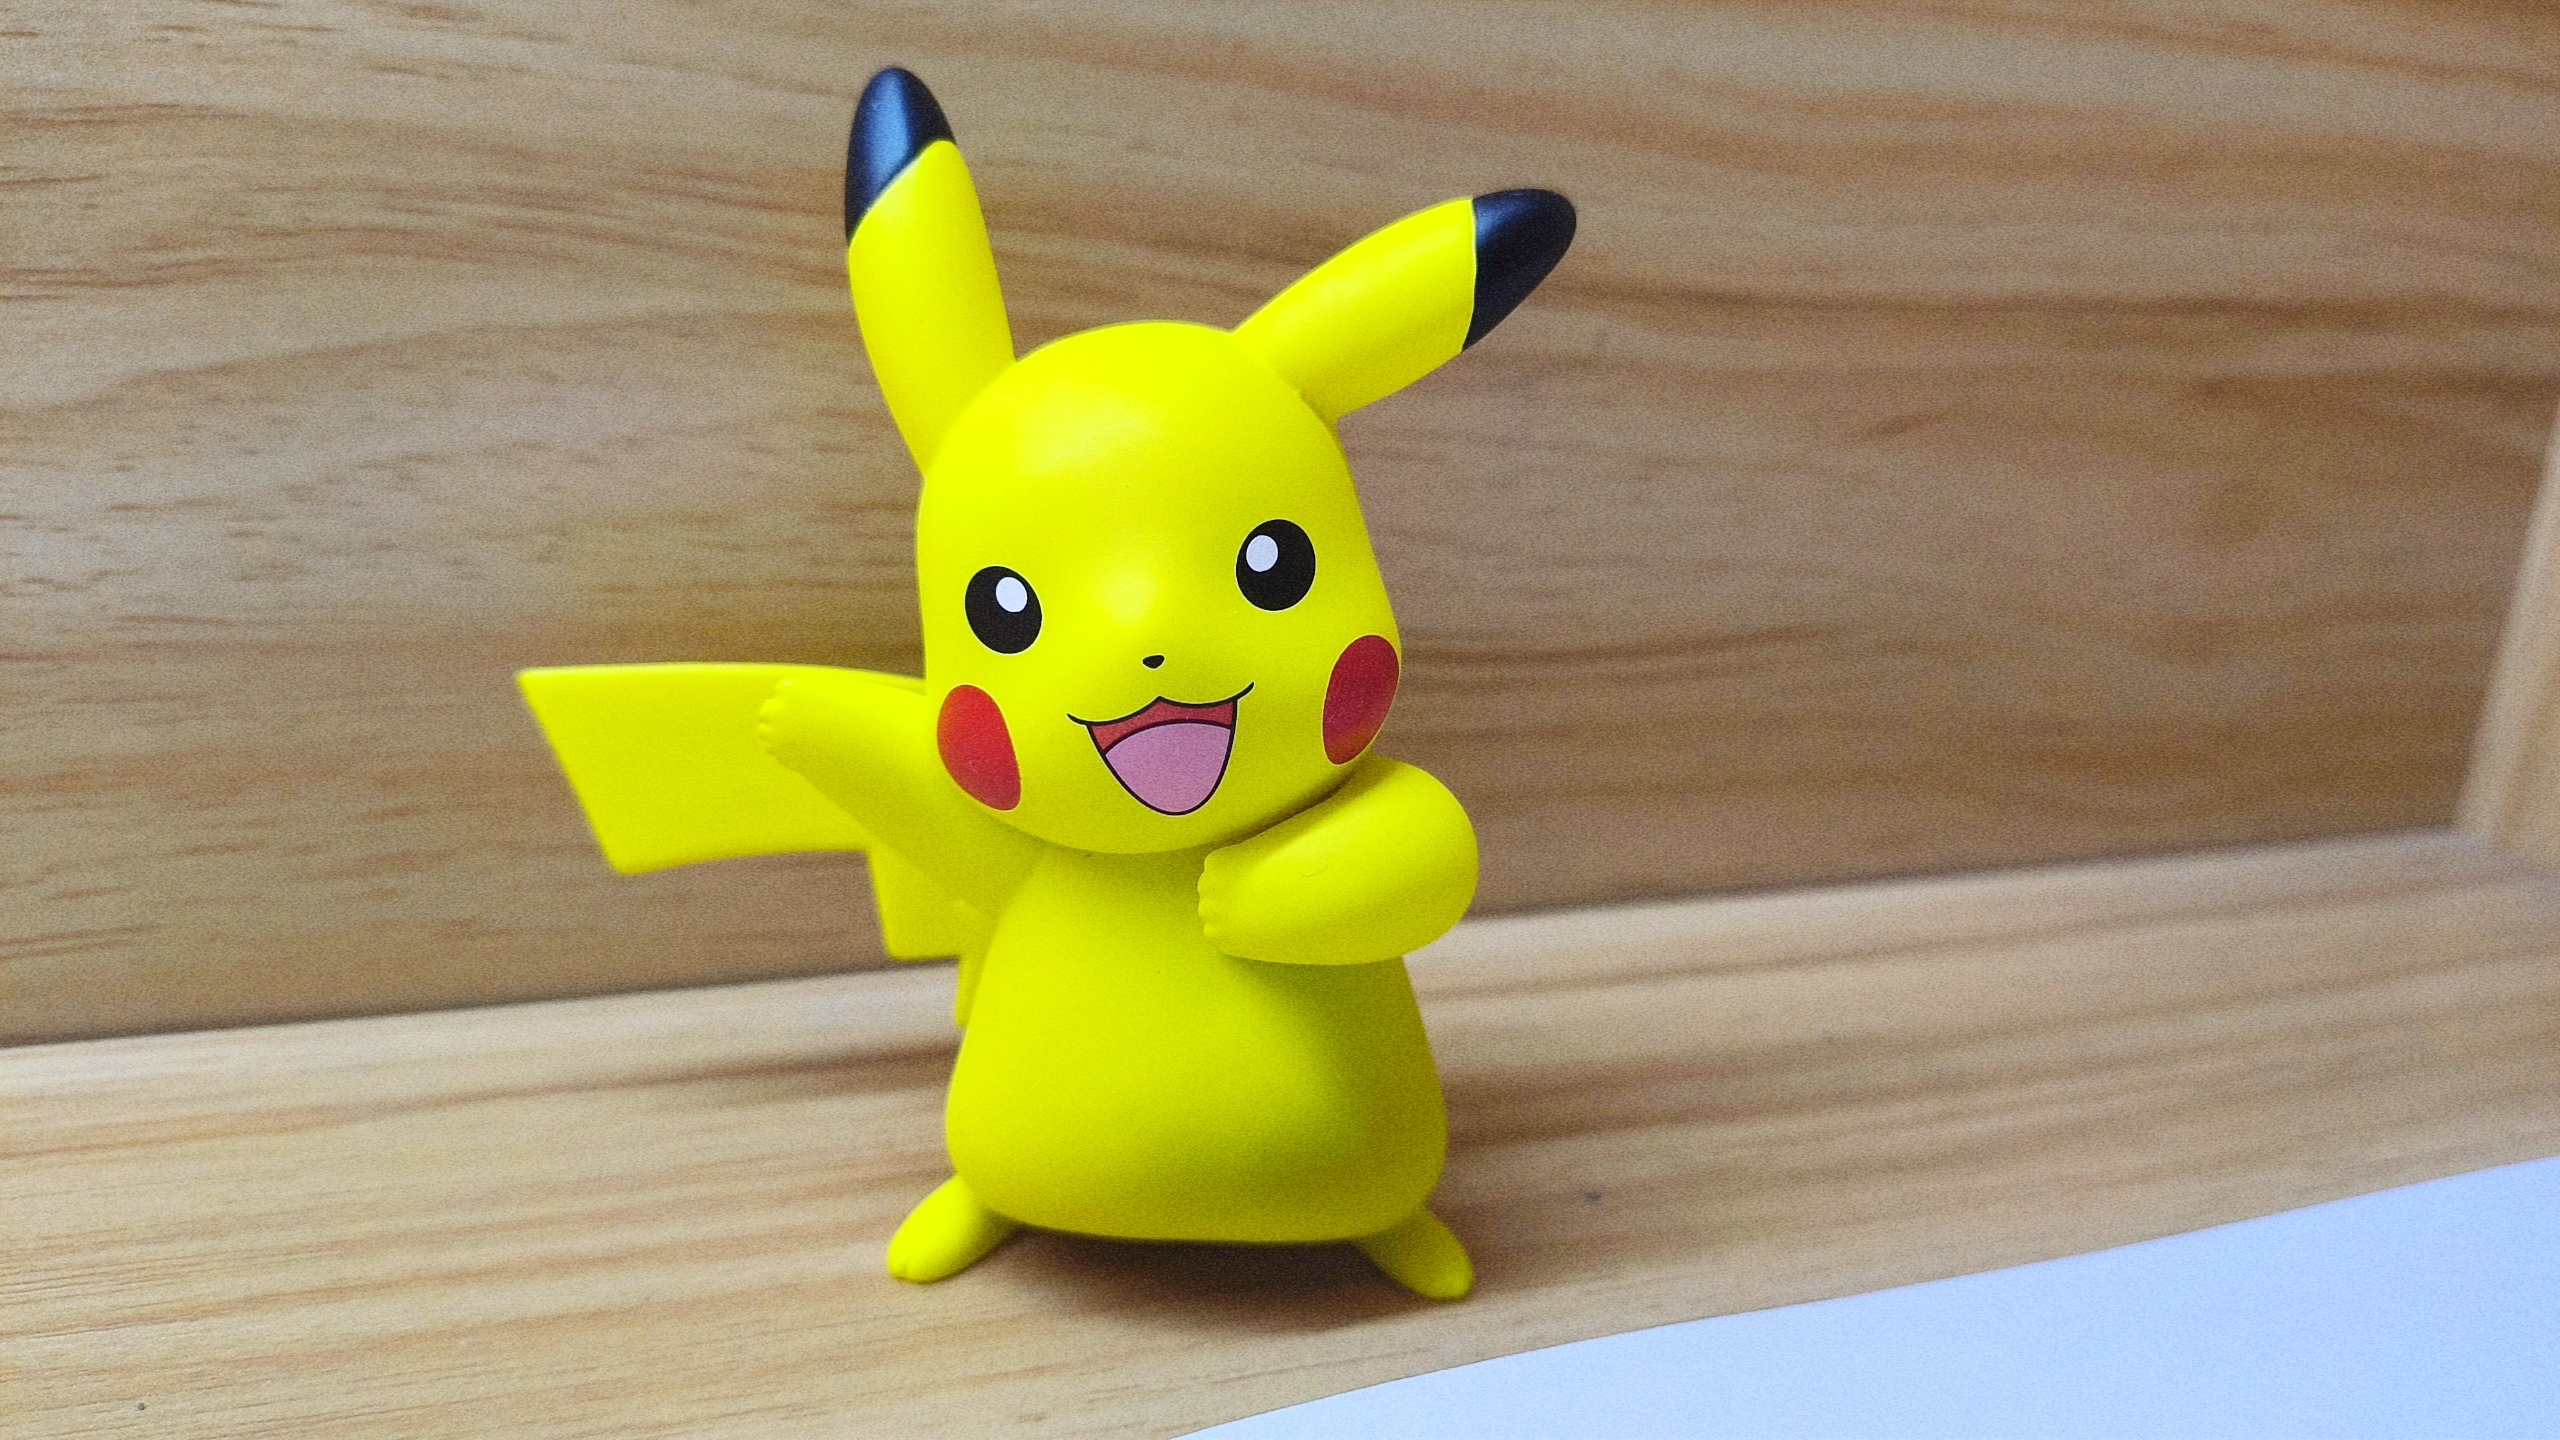
\includegraphics[scale=0.1]{figures/pikachu.jpg}
        \caption{这是图片}
        \label{fig:2}
    \end{figure}
    \subsubsection{表格}
    \begin{table}[!htbp]
        \centering
        \caption{这是表格}
        \begin{tabular}{cccccc}
            \toprule
            序号 & 姓名 & 性别 & 年龄 & 身高/cm & 体重/kg \\
            \midrule
            1 & 张三 & M & 16 & 163 & 50 \\
            2 & 王红 & F & 15 & 159 & 47 \\
            3 & 李二 & M & 17 & 165 & 52 \\
            \bottomrule
        \end{tabular}
        \label{tab:2}
    \end{table}
    \subsubsection{代码块}
    \begin{lstlisting}
        #include <stdio.h>
        /* hello,world */
        int main(){
            printf("Hello, World! \n"); 
            return 0;
        }
    \end{lstlisting}
    \subsection{数学公式}
    \subsubsection{行内公式}
    这是简单的行内公式:$x^2+y^2=z^2$,这是复杂的行内公式:$\sum_{i=1}^n a_i=0$。
    \subsubsection{行间公式}
    (1)线性代数部分:
    \begin{equation}
        \begin{split}
            \mathbf{A}\mathbf{x} &= \mathbf{b} \\
            \mathbf{A}^{-1}\mathbf{A}\mathbf{x} &= \mathbf{A}^{-1}\mathbf{b} \\
            \mathbf{I}\mathbf{x} &= \mathbf{A}^{-1}\mathbf{b} \\
            \mathbf{x} &= \mathbf{A}^{-1}\mathbf{b}
        \end{split}
    \end{equation}

    (2)微积分部分:
    \begin{equation}
        \begin{split}
            \frac{d}{dx} \int_a^x f(t)\,dt &= f(x) \label{eq:2} \\
            \int_a^b f(x)\,dx &= F(b)-F(a)
        \end{split}
    \end{equation}

    (3)概率论部分:
    \begin{equation}
        \begin{split}
            P(A \mid B) &= \frac{P(A \cap B)}{P(B)} \\
            &= \frac{P(B \cap A)}{P(B)} \\
            &= \frac{P(B \mid A)P(A)}{P(B)}
        \end{split}
    \end{equation}

    (4)统计部分:
    \begin{equation}
        \begin{split}
            \bar{x} &= \frac{1}{n}\sum_{i=1}^n x_i \\
            s^2 &= \frac{1}{n-1}\sum_{i=1}^n (x_i-\bar{x})^2 \\
            s &= \sqrt{s^2}
        \end{split}
    \end{equation}

    (5)离散数学部分:
    \begin{equation}
        \begin{split}
            \binom{n}{k} &= \frac{n!}{k!(n-k)!} \\
            \binom{n}{0} &= \binom{n}{n} = 1 \\
            \binom{n}{1} &= \binom{n}{n-1} = n \\
            \binom{n}{2} &= \binom{n}{n-2} = \frac{n(n-1)}{2} \\
            \binom{n}{k} &= \binom{n}{n-k}
        \end{split}
    \end{equation}

    (6)其他部分:
    \begin{equation}
        \begin{split}
            \log_a x &= \frac{\log_b x}{\log_b a} \\
            \log_a x &= \frac{\log_c x}{\log_c a} \\
            \log_a x &= \frac{\log_a b}{\log_a c} \\
            \log_a x &= \frac{\log_b x}{\log_b c}
        \end{split}
    \end{equation}
    \section{交叉引用}\label{sec:3}
    \subsection{参考文献引用}\label{sec:4}
    这是第一个参考文献的交叉引用\cite{shannon1948mathematical}。

    这是第二个参考文献的交叉引用\cite{nash1996non}。

    这是第三个参考文献的交叉引用\cite{turing2009computing}。
    \subsection{图表引用}
    这是图片\ref{fig:2}的交叉引用。

    这是表格\ref{tab:2}的交叉引用。
    \subsection{章节引用}
    这是章节\ref{sec:3}的交叉引用。

    这是章节\ref{sec:4}的交叉引用。
    \subsection{公式引用}
    这是公式\ref{eq:2}的交叉引用。
\end{ujnbody}